\ifx\wholebook\relax \else

\documentclass[b5paper]{ctexart}
\usepackage[nomarginpar
  %, margin=.5in
]{geometry}

\addtolength{\oddsidemargin}{-0.05in}
\addtolength{\evensidemargin}{-0.05in}
\addtolength{\textwidth}{0.1in}

\usepackage[cn]{../prelude}

\setcounter{page}{1}

\begin{document}

\title{数的诞生}

\author{刘新宇
\thanks{{\bfseries 刘新宇} \newline
  Email: liuxinyu99@hotmail.com \newline}
  }

\maketitle
\fi

\markboth{数的诞生}{数的旅程}

\ifx\wholebook\relax
\chapter{数的诞生}
\numberwithin{Exercise}{chapter}
\fi

\epigraph{一二三四五,金木水火土。\\
天地分上下,日月照今古。}{部编小学一年级\\
语文课本第一课}

数充满了我们的生活。例如报纸上这段新闻报道:“2024年巴黎奥运会(第33届奥运会)已于当地时间2024年8月1日闭幕。巴黎是继伦敦后的世界第2个至少3次举办夏奥会的城市。这是首届男女比例完全平衡的奥运会,男女运动员各为5250名。本届奥运会共设有32个大项,329个小项,共有206个国家和地区参赛,新增了滑板、冲浪、竞技攀岩和霹雳舞四个大项。中国代表团最终在巴黎奥运会上夺得40金27银24铜的优异成绩。”

这短短的180字中有14个数字。数是谁发明的?历史书上没有答案。数出现在所有历史文字记录中,数也许诞生在史前,伴随着语言和文字。要找到答案,我们有两条线索:1、追寻古老的历史物证,石刻、壁画、器物上关于数的印记;2、追溯数在语言演变中的痕迹。比如英文中的eleven (11)来自古英语endleofan,意思是(数到10还)剩余1;tweleve (12)来自twelf,意思是剩余2。

\section{罗塞塔石碑}
\index{罗塞塔石碑}

\begin{figure}[htbp]
 \centering
 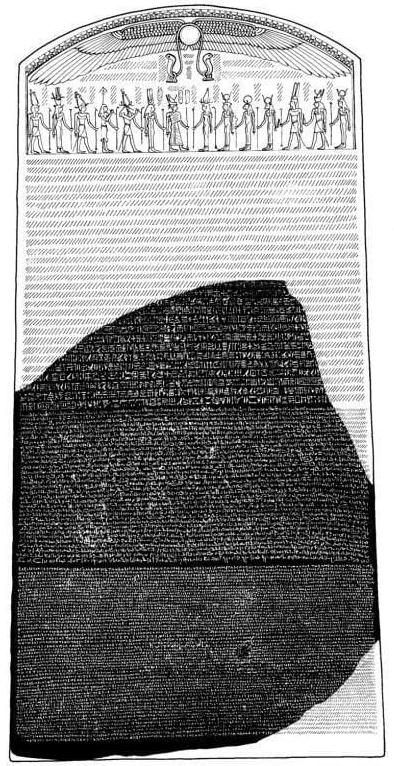
\includegraphics[scale=1.0]{img/Rosetta-stone-recons}
 \caption{古埃及罗赛塔石碑。石碑不完整,从中间断裂。}
 \label{fig:rosetta-stone-recons}
\end{figure}

走进大英博物馆第4展厅,有一件展品吸引着观众。这是一块残缺的石碑,长114厘米,宽72厘米,上面刻满了文字(\cref{fig:rosetta-stone-recons})。人们能一眼辨认出位于底部的内容是希腊字母(\cref{fig:rosetta-greek},参见\cref{ch:greek-letters}希腊字母表),但上面的部分犹如天书。仔细观察会发现余下的文字大致分成两种:一种是弯弯曲曲的符号,如\cref{fig:rosetta-demotic},位于石碑中部;另一种是奇妙的图案,如\cref{fig:rosetta-hieroglyphs},位于石碑上部。

\begin{figure}[htbp]
  \centering
  \subcaptionbox{古希腊文,共54行\label{fig:rosetta-greek}}{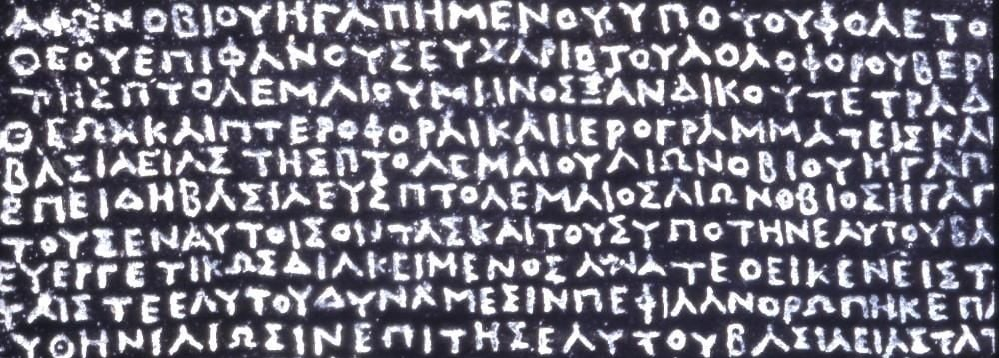
\includegraphics[scale=0.5]{img/Rosetta-Greek}} \\
  \subcaptionbox{古埃及世俗文字,是当时埃及平民使用的文字。共32行\label{fig:rosetta-demotic}}{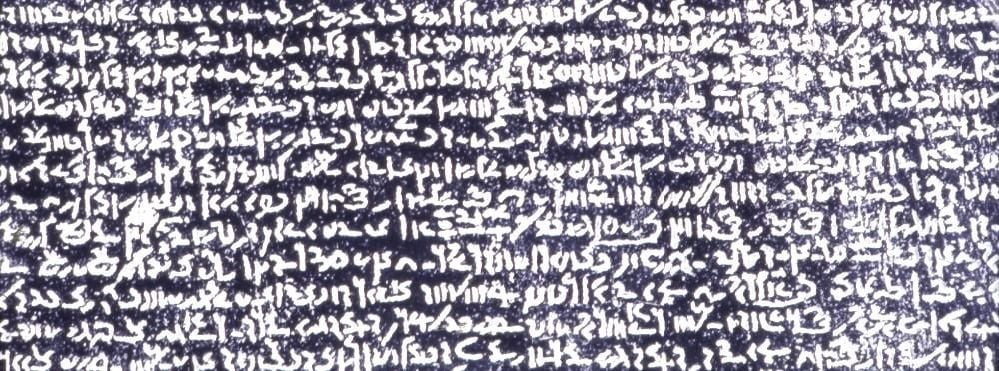
\includegraphics[scale=0.5]{img/Rosetta-Demotic}} \\
  \subcaptionbox{古埃及象形文字,又称圣书体,代表献给神明的文字。共14行\label{fig:rosetta-hieroglyphs}}{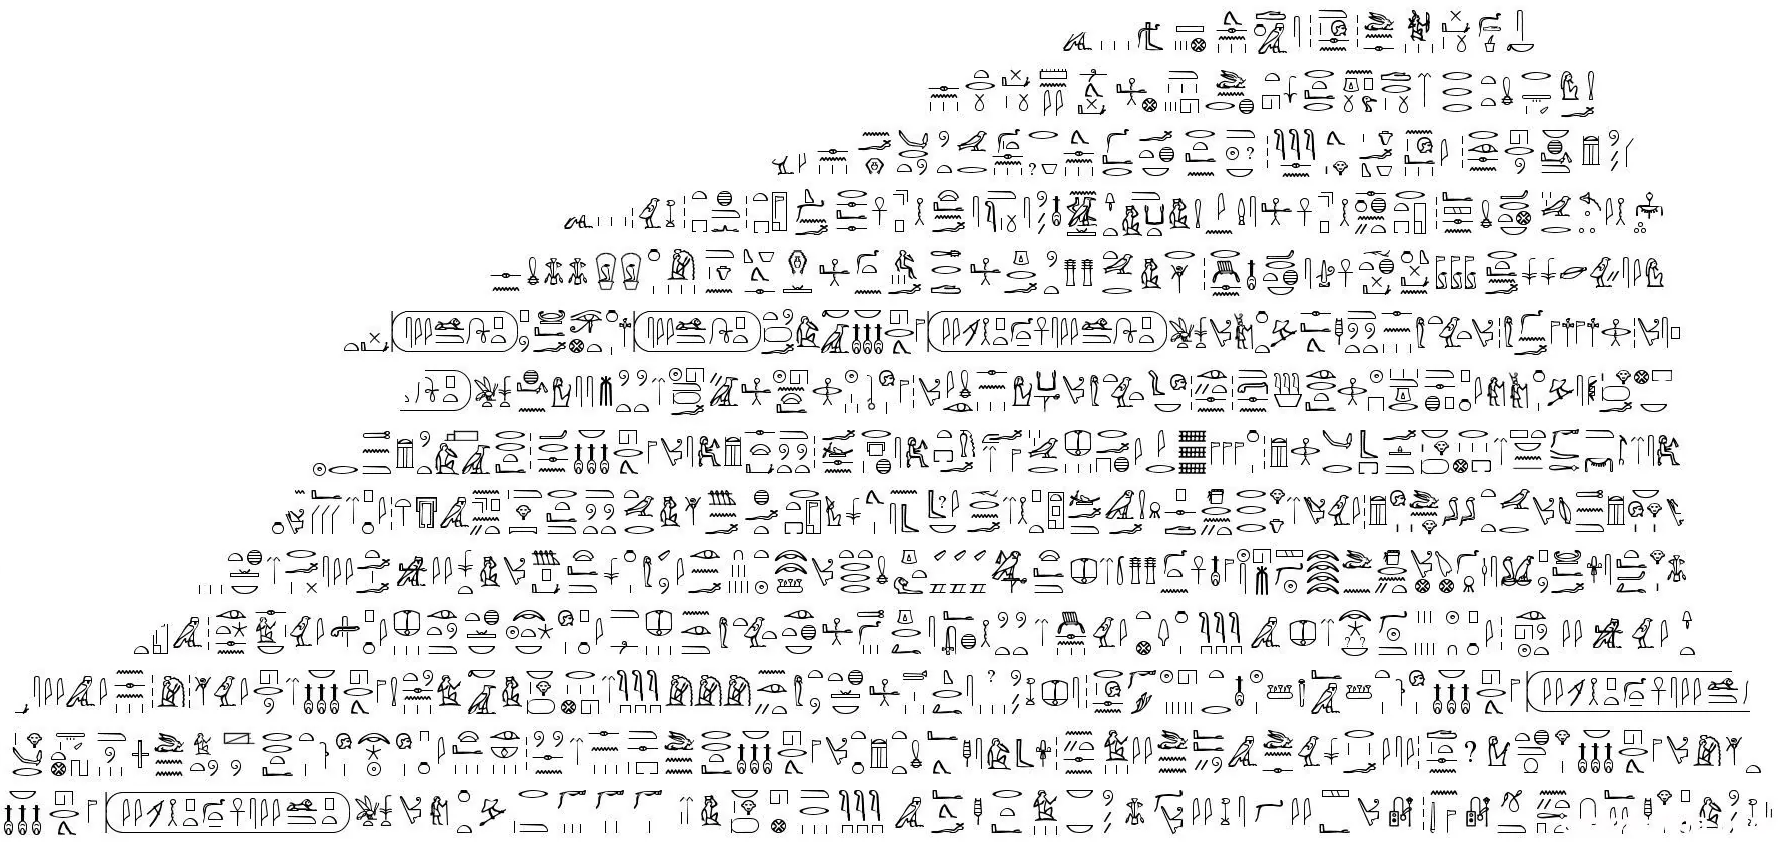
\includegraphics[scale=0.3]{img/Rosetta-Hieroglyphs-c}}
  \caption{罗赛塔石碑上的三种文字}
  \label{fig:rosetta-stone}
 \end{figure}

这一展品叫做罗塞塔石碑。1799年,拿破仑率领法军远征埃及。远征军有3万余人,各类舰只350艘,另有学者工程师146人。这位未来的法兰西皇帝从一名炮兵军官脱颖而出。他敏锐地看出数学不仅可以算出大炮的弹道,还关乎法兰西的国运。拿破仑的大军巧妙地避开了英国海军的封锁,7月2日攻占了埃及的亚历山大城,随即向开罗进军。7月15日,一位士兵在尼罗河三角洲前线的小镇罗塞塔(Rosetta)挖掘防御工事。他偶然发现了一块断碑砌在一段古老的墙中。尽管并不完整,这仍是一个重大的发现。法军指挥官决定把它送到拿破仑设立于开罗的埃及研究所,并于8月运抵开罗。根据发现地点,它被命名为罗塞塔石碑。1801年,英军击败了拿破仑,罗塞塔石碑也落入了英军之手。1802年2月,它被运抵英国朴次茅斯港,并最终收藏于大英博物馆。

这块石碑有何特殊之处呢?它上面用三种不同的文字记录了同一内容:公元前196年,13岁的国王托勒密5世加冕一周年。他从父亲托勒密4世袭得正统王位,并做了许多善行,如捐助神庙、减免税收等等。埃及当时处于托勒密王朝的统治之下,统治者是希腊人\footnote{马其顿国王亚历山大大帝征服了埃及。他死后,埃及总督托勒密一世与公元前305年自称国王建立王朝,统治埃及275年。}。国王宣称自己是法老。因此铭文使用了古埃及象形文字、古埃及世俗文字、希腊官方文字三种文字镌刻,并颁布全埃及各个神庙勒石立碑。而罗塞塔石碑就是其中之一,并且是至今唯一发现的一块。罗塞塔石碑于是成为了破解古埃及文字的钥匙。英国物理学家托马斯·杨(1773~1829,就是高中物理课本中杨氏双缝实验——发现光的干涉现象的物理学家)和法国学者商博良通过研究此碑,成功破译了古埃及象形文字。

\section{计数系统}
\index{计数系统}

通过对古文字的破译,我们发现古埃及大约在公元前3400年就出现了表示数字的符号。是众多古文明中最早的(美索不达米亚大约在公元前3000年出现了数字符号,中国大约在公元前1600年出现了数字符号)。各文明中最早出现的数字符号是多是“|”、“||”、“||”或“-”、“=”、“$\equiv$”。这表明我们的老祖先是从“数数”开始认识数字的。很可能是采集、狩猎到更多的东西。随着生产生活的进步,人们逐渐认识更大的数,并逐渐从一数到了十——显然我们的祖先搬着手指头数数。但接下来遇到了困难。人只有两只手十个手指。这时有三种解决方法:(1)把脚也用上可以数到二十,但接下来会遇到同样的问题。(2)自由分组。在西伯利亚的尤卡吉尔语中有这样的例子:三和一、两个三、两个四、十差一等等。(3)固定分组。数到某一固定数目,例如十,分成一组,把这个组看成一个单位并起个名字。比如古埃及用$\cap$表示十。这样$\cap \cap$表示二十(古罗马用X表示十,I表示一。23表示为XXIII)。

为了建造宏伟的金字塔,古埃及人还创造了更大的单位符号,如\cref{fig:egypt-hieroglyphic-numerals}。他们用永恒之神(Heh)代表一百万,用蝌蚪表示十万,用弯曲的手指表示一万,莲花表示一千、弯曲的绳子表示一百……

\begin{figure}[htbp]
 \centering
 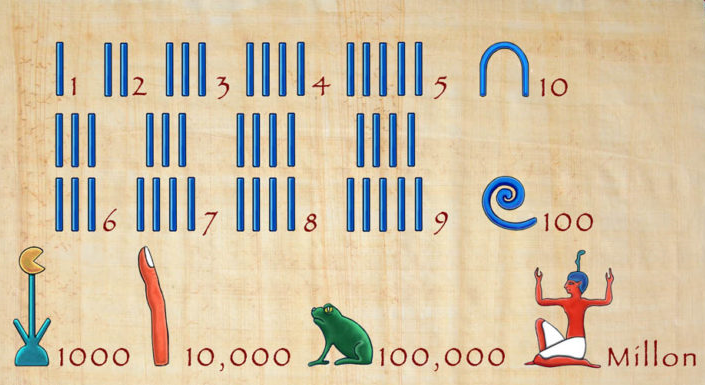
\includegraphics[scale=0.8]{img/hieroglyphic-numbers}
 \caption{古埃及象形文字中的数字符号。}
 \label{fig:egypt-hieroglyphic-numerals}
\end{figure}

计数时按照单位分组,超出后就组成更大的单位。最后把每个单位的数目和单位表示的大小乘起来。\cref{fig:egypt-number-examples}给出了两个例子。尽管这种方法能够处理很大的数,但方法(2)自由分组对付小数字也很方便。古巴比伦人使用60进制(分组单位是60)。这种进制今天也出现在我们的日常生活中。60秒是1分,60分是1小时。所以1小时12分30秒,或写成1:12:30,包括$1(60\times 60) + 12(60) + 30 = 4350$秒。60对古巴比伦人足够大,所以他们在60以内使用自由分组法,超过60用$60^2$、$60^3$、$60^4$……分组,如\cref{fig:babylonian-numerals}。

\begin{figure}[htbp]
 \centering
 \subcaptionbox{数字214427表示为$2(100000)+1(10000)+4(1000)+4(100)+2(10)+7(1)$}{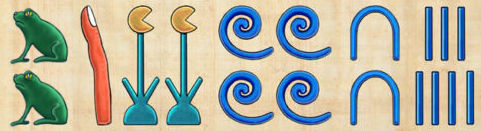
\includegraphics[scale=0.5]{img/egypt-num-eg2}}
 \subcaptionbox{古埃及埃德富(Edfu)神庙中的象形文字数字。表示1333330}{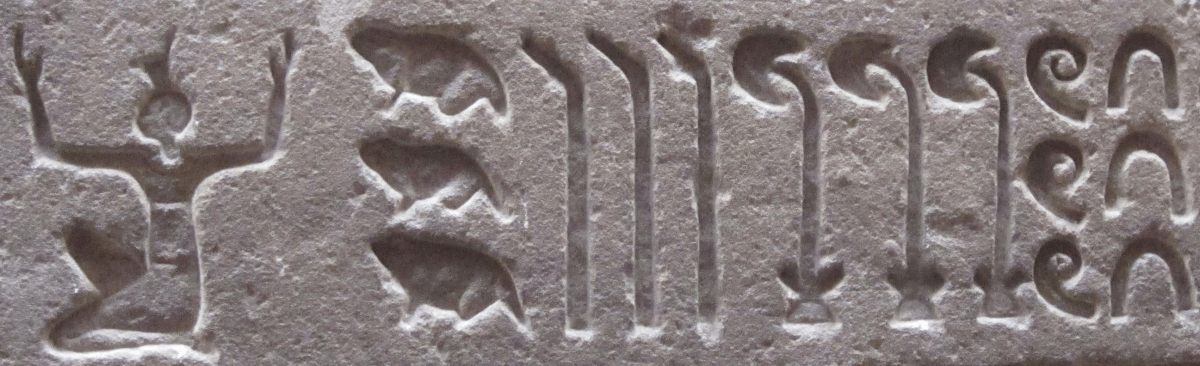
\includegraphics[scale=0.2]{img/Hieroglyphic-num-eg}}
 \caption{古埃及象形文字数字的例子}
 \label{fig:egypt-number-examples}
\end{figure}

\begin{figure}[htbp]
 \centering
 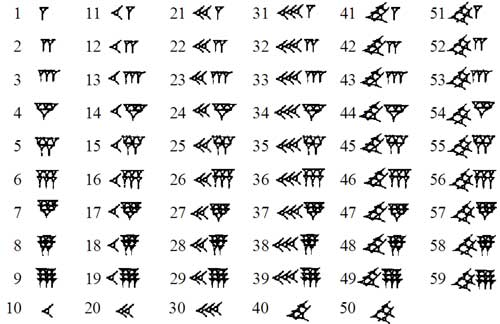
\includegraphics[scale=1.0]{img/Babylonian-numerals}
 \caption{古巴比伦楔形文字中的数字符号。}
 \label{fig:babylonian-numerals}
\end{figure}


\ifx\wholebook\relax \else
\section{参考答案}
\shipoutAnswer

\begin{thebibliography}{99}

%% \bibitem{wiki-number}
%% Wikipedia. ``古代计数系统的历史''. \url{https://en.wikipedia.org/wiki/History_of_ancient_numeral_systems}

%% \bibitem{trip-to-number-kingdom}
%% [美]\ 卡尔文$\cdot$C$\cdot$克劳森\ 著\ 袁向东、袁钧\ 译. ``数学旅行家:漫游数王国''. 上海教育出版社。ISBN: 7-5320-7883-3/G $\cdot$ 7972

%% \bibitem{wiki-babylonian-num}
%% Wikipedia. ``古巴比伦数字''. \url{https://en.wikipedia.org/wiki/Babylonian_numerals}

\end{thebibliography}

\expandafter\enddocument
%\end{document}

\fi
